\section{Question 1: Encoding and generating Meowdoku grids}\label{sec:q1}

\begin{center}
\begin{tabular}{@{}p{6.2cm}p{10cm}@{}}
\toprule
File & Description\\
\midrule
\texttt{image\_grid.txt} & The board of Figure~\ref{fig:meowdoku-board} in the grid-file format of the assignment (\texttt{GRID}, \texttt{ZONES}, then one line of region labels per row). Input of the converter.\\
\texttt{meowdoku\_to\_dimacs.py} & Converter from a grid file to a DIMACS CNF file: \texttt{read\_grid}, \texttt{encode\_grid} and \texttt{write\_dimacs}.\\
\texttt{generate\_grid.py} & Generator of square boards with a planted solution: \texttt{cat\_columns} plants the cats, \texttt{generate\_grid} grows the regions, and \texttt{write\_grid} writes the grid file.\\
\bottomrule
\end{tabular}
\end{center}

\subsection{The board and its variables}

A Meowdoku grid has $N$ rows, $M$ columns, and $K$ disjoint colored regions. A legal placement has at most one cat in each row and column, exactly one cat in each region, and no two cats in cells that touch along an edge or corner. Figure~\ref{fig:meowdoku-board} is the single running example in this report; ``the board'' below always refers to it. It has $N=M=K=6$, and its six cats show a complete legal placement. The SAT input uses the colored regions; the cats of Figure~\ref{fig:meowdoku-board} illustrate a solution rather than fixed clues in the input file.

\begin{figure}[htbp]
\centering
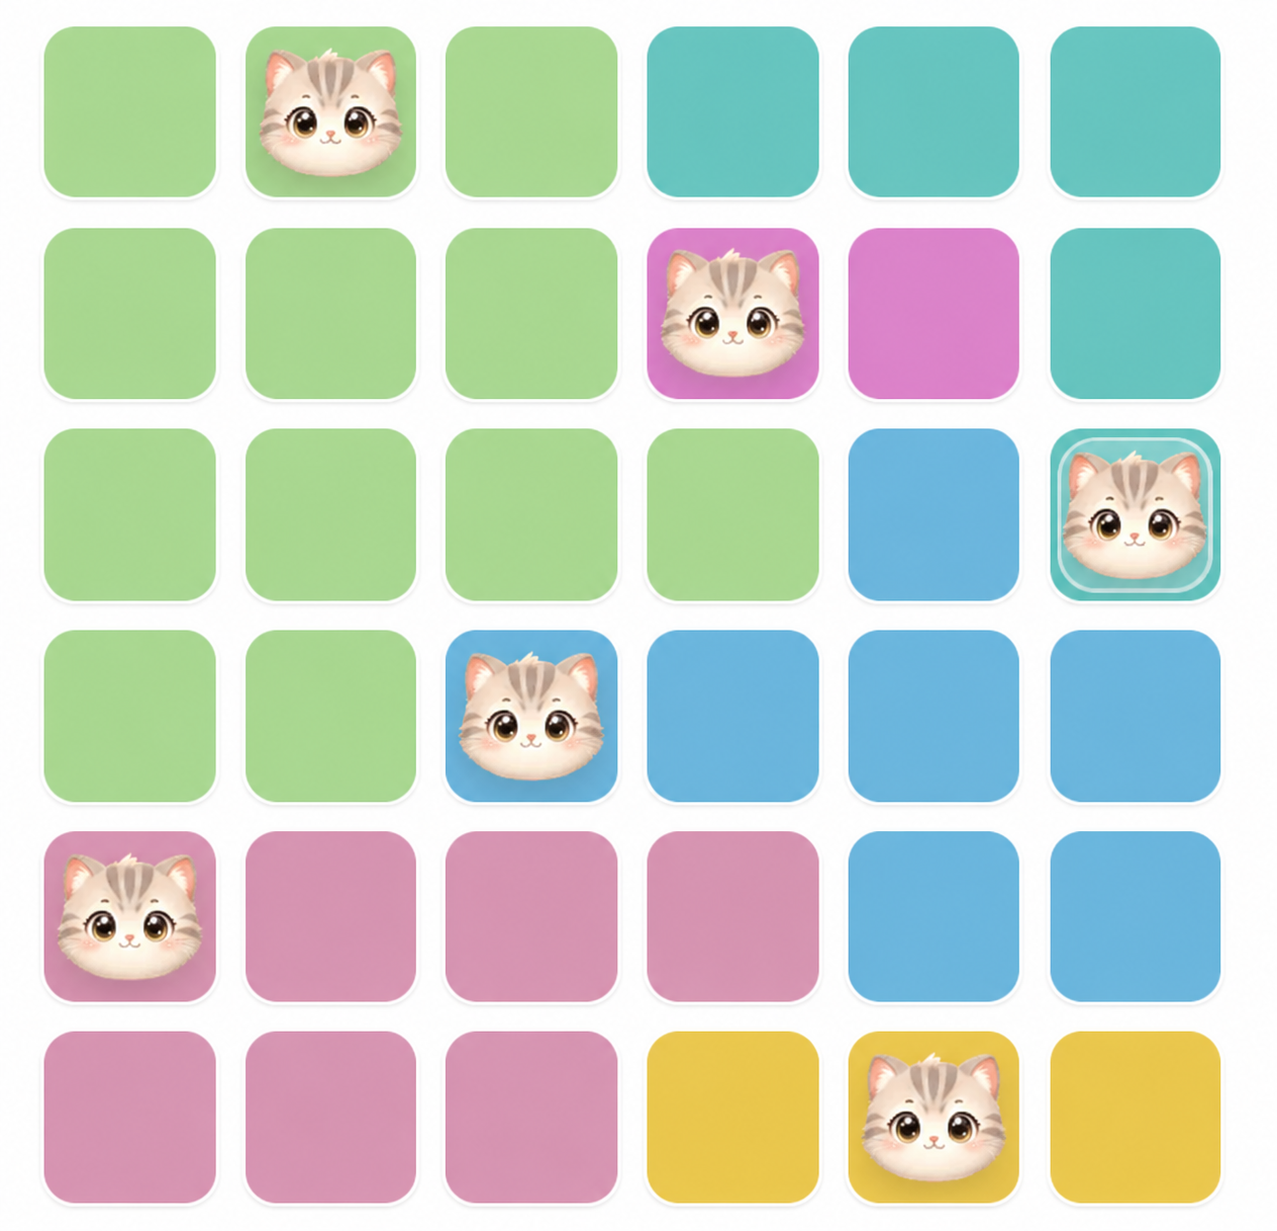
\includegraphics[width=0.55\linewidth]{figures/meowdoku_board.png}
\caption{Example of a $6\times6$ Meowdoku board. Colors define the six regions, and the six cats show a complete solution.}
\label{fig:meowdoku-board}
\end{figure}

We name the green, turquoise, pink, blue, mauve, and yellow regions A, B, C, D, E, and F, respectively. The colors give the following complete grid description, saved as \texttt{image\_grid.txt}:
\begin{verbatim}
GRID 6 6
ZONES A B C D E F

A A A B B B
A A A C C B
A A A A D B
A A D D D D
E E E E D D
E E E F F F
\end{verbatim}
Each of the six final lines describes one row, from top to bottom; each label identifies the region of one cell, from left to right. Thus the pink region is $R_C=\{(2,4),(2,5)\}$, whereas the green region includes cells in four different rows. The file records regions, not cat positions. Let $R_A,\ldots,R_F$ denote the sets of cells carrying the corresponding labels. These six nonempty sets partition all 36 cells. In formulas indexed by $r=1,\ldots,K$, we identify $R_1=R_A,\ldots,R_6=R_F$.

For every cell $(i,j)$, with row $i$ and column $j$ numbered from 1, introduce a Boolean variable $x_{i,j}$. It is true exactly when a cat is in that cell. A negative literal $\neg x_{i,j}$ means that the cell is empty. DIMACS represents each variable with an integer:
\[
\operatorname{id}(i,j)=(i-1)M+j=(i-1)6+j.
\]
The first term skips the $i-1$ preceding rows of six cells; adding $j$ selects the cell in row $i$. For example, the cat in pink cell $(2,4)$ corresponds to $\operatorname{id}(2,4)=(2-1)6+4=10$, so its variable is $x_{2,4}$ and its DIMACS positive literal is \texttt{10}. The yellow cat in $(6,5)$ has variable number $(6-1)6+5=35$. All 36 cells have distinct IDs from 1 to 36:
\[
\begin{array}{c|rrrrrr}
 & j=1&j=2&j=3&j=4&j=5&j=6\\ \hline
 i=1&1&2&3&4&5&6\\
 i=2&7&8&9&10&11&12\\
 i=3&13&14&15&16&17&18\\
 i=4&19&20&21&22&23&24\\
 i=5&25&26&27&28&29&30\\
 i=6&31&32&33&34&35&36
\end{array}.
\]

The following table lists every variable belonging to each region. It is equivalent to the colored grid because the preceding formula converts every listed ID back to a unique cell.
\begin{center}
\begin{tabular}{@{}lp{9cm}r@{}}
\toprule
Region & Cell-variable IDs & $s_r=|R_r|$\\
\midrule
A (green) & 1, 2, 3, 7, 8, 9, 13, 14, 15, 16, 19, 20 & 12\\
B (turquoise) & 4, 5, 6, 12, 18 & 5\\
C (pink) & 10, 11 & 2\\
D (blue) & 17, 21, 22, 23, 24, 29, 30 & 7\\
E (mauve) & 25, 26, 27, 28, 31, 32, 33 & 7\\
F (yellow) & 34, 35, 36 & 3\\
\bottomrule
\end{tabular}
\end{center}

The six cats in Figure~\ref{fig:meowdoku-board} occupy $(1,2)$, $(2,4)$, $(3,6)$, $(4,3)$, $(5,1)$, and $(6,5)$, with IDs $2$, $10$, $18$, $21$, $25$, and $35$. The corresponding satisfying assignment sets exactly
\[
T=\{x_{1,2},x_{2,4},x_{3,6},x_{4,3},x_{5,1},x_{6,5}\}
\]
to true and all other cell variables to false. The six cats occupy different rows, columns, and regions. Their column sequence $2,4,6,3,1,5$ has gaps greater than one between consecutive rows, so none touch diagonally.

\subsection{From an expression to DIMACS}

A \emph{literal} is a variable or its negation. Literals joined by $\lor$ (OR) form a \emph{clause}; clauses joined by $\land$ (AND) form a formula in \emph{conjunctive normal form} (CNF). Every clause must be true. The symbols $\bigvee$ and $\bigwedge$ repeat OR and AND over the indices written below them. A comma in an index lists simultaneous conditions; it is not itself a logical operator.

The pink region has only the cells $(2,4)$ and $(2,5)$. Requiring exactly one cat there gives the small CNF fragment
\[
\underbrace{(x_{2,4}\lor x_{2,5})}_{\text{at least one}}
\land
\underbrace{(\neg x_{2,4}\lor\neg x_{2,5})}_{\text{at most one}}.
\]
Their IDs are 10 and 11. As a standalone two-clause fragment using the board's 36 variable numbers, the expression becomes
\begin{verbatim}
p cnf 36 2
10 11 0
-10 -11 0
\end{verbatim}
In general, the DIMACS header has the form \texttt{p cnf V C}: $V$ is the number of Boolean \emph{variables}, and $C$ is the number of clauses that follow. There is one variable per cell, so the board has $V=NM=6\cdot6=36$. The two clauses above are only a fragment of the complete formula, hence $C=2$ in this example. Each OR-clause becomes one line, and placing both lines in the file represents AND. A positive number denotes a variable and a negative number its negation. Zero ends a clause; it is a delimiter, not variable zero or the Boolean value false.

The complete board formula contains additional clauses for all four rules, each written in the same DIMACS format.

\subsection{The four rules as clauses}

\subsubsection{At most one cat in each row}

For distinct cells $(i,j)$ and $(i,k)$ in the same row, at least one must be empty. The clause $\neg x_{i,j}\lor\neg x_{i,k}$ is false precisely when both contain cats. We write it for every pair of columns $j<k$ in every row $i$:
\[
F_{\mathrm{rows}}=
\bigwedge_{1\le i\le N,\;1\le j<k\le M}
\underbrace{(\neg x_{i,j}\lor\neg x_{i,k})}_{\text{not both cats in row }i}.
\]
For example, in the first row, cells $(1,2)$ and $(1,3)$ have IDs 2 and 3. Their clause becomes \texttt{-2 -3 0}. The cat at $(1,2)$ makes $x_{1,2}$ true, so the clause requires $x_{1,3}$ to be false. We need a clause for every pair, since excluding only this pair would still allow cats at other two cells of the row. The condition $j<k$ visits each unordered pair once and never pairs a cell with itself. These clauses allow zero or one cat in a row, exactly as the rule states.

\subsubsection{At most one cat in each column}

Two cells in one column have the same $j$ and different row numbers $i<k$. Applying the same pairwise exclusion gives
\[
F_{\mathrm{columns}}=
\bigwedge_{1\le j\le M,\;1\le i<k\le N}
\underbrace{(\neg x_{i,j}\lor\neg x_{k,j})}_{\text{not both cats in column }j}.
\]
In column 4, the cat at $(2,4)$ has ID 10, while yellow cell $(6,4)$ has ID 34. The clause $\neg x_{2,4}\lor\neg x_{6,4}$ becomes \texttt{-10 -34 0}. Since the cat at $(2,4)$ makes the first literal false, $(6,4)$ must remain empty. The rule covers any two cells in a column, even if they are not adjacent.

\subsubsection{Exactly one cat in each region}

For a region $R_r$, one positive clause requires at least one cat. Negative clauses for all pairs of distinct cells prevent a second cat. Both conditions must hold for every region:
\[
F_{\mathrm{regions}}=
\bigwedge_{1\le r\le K}
\left[
\underbrace{\left(\bigvee_{u\in R_r}x_u\right)}_{\text{at least one cat}}
\land
\underbrace{\left(\bigwedge_{\{u,v\}\in\binom{R_r}{2}}
(\neg x_u\lor\neg x_v)\right)}_{\text{at most one cat}}
\right].
\]
Here $u$ and $v$ are cells, $x_u$ is the variable of cell $u$, and $\binom{R_r}{2}$ denotes all unordered pairs of different cells in that region. The inner $\bigwedge$ makes one negative clause per pair; the outer $\bigwedge$ repeats the entire requirement for A through F. The pink region C gives exactly the two DIMACS lines shown above: \texttt{10 11 0} and \texttt{-10 -11 0}. The positive line rules out an empty pink region; the negative line rules out two pink cats. The cat at $(2,4)$ satisfies the first and forces $(2,5)$ to be empty through the second. A larger region, such as yellow F with IDs 34, 35, and 36, has the positive line \texttt{34 35 36 0} and three pair lines \texttt{-34 -35 0}, \texttt{-34 -36 0}, and \texttt{-35 -36 0}.

\subsubsection{No two cats in adjacent cells}

The game's eight-neighbor rule includes horizontal, vertical, and diagonal contact. The row clauses already exclude every horizontal pair, and the column clauses exclude every vertical pair. To cover diagonal contact, consider each $2\times2$ block and forbid its two diagonals:
\[
F_{\mathrm{diagonals}}=
\bigwedge_{1\le i<N,\;1\le j<M}
\left[
\underbrace{(\neg x_{i,j}\lor\neg x_{i+1,j+1})}_{\text{first diagonal pair}}
\land
\underbrace{(\neg x_{i,j+1}\lor\neg x_{i+1,j})}_{\text{second diagonal pair}}
\right].
\]
For the block comprising rows 1--2 and columns 3--4, the first diagonal pair has IDs 3 and 10, giving \texttt{-3 -10 0}; the second diagonal pair has IDs 4 and 9, giving \texttt{-4 -9 0}. Because the cat at $(2,4)$ makes $x_{2,4}$ true, the first clause forbids a cat at $(1,3)$. Every diagonally touching pair belongs to such a block, so iterating over all blocks covers the entire grid without extra clauses for horizontal or vertical adjacency.

The complete formula is
\[
F=F_{\mathrm{rows}}\land F_{\mathrm{columns}}
\land F_{\mathrm{regions}}\land F_{\mathrm{diagonals}}.
\]
For a general $N\times M$ board, rows and columns are constrained by \emph{at most} one, not necessarily exactly one. On this board, $N=M=K=6$ and the six region clauses require six cats. Since six rows and six columns can hold at most six cats, each must in fact contain exactly one.

\subsection{From a grid text file to a CNF file}

The converter (\texttt{meowdoku\_to\_dimacs.py}) turns a grid file into a DIMACS CNF file in three phases: it reads and checks the grid, it generates the clauses of the four rules, and it writes them out. The procedure below uses the notation of the previous sections: $\operatorname{reg}(i,j)$ is the region label of cell $(i,j)$, and a clause is written as a set of DIMACS literals, that is, nonzero integers whose sign is the polarity.

\begin{pseudo}{Procedure: grid file to DIMACS CNF}
\pinfo{\textbf{Input:} a grid file. \textbf{Output:} a DIMACS CNF file.}
\pline{0}{ignore blank lines and comment lines (those starting with \texttt{c})}
\pline{0}{read $N$ and $M$ from the line \texttt{GRID $N$ $M$} and the region names from the line \texttt{ZONES}}
\pline{0}{read the next $N$ lines, each made of $M$ labels; $\operatorname{reg}(i,j)\leftarrow$ the label in row $i$, column $j$}
\pline{0}{\kw{if} the names are not distinct, the numbers of rows or labels are wrong, or the labels used are not exactly the declared names \kw{then} reject the file}
\pline{0}{$\operatorname{id}(i,j)\leftarrow(i-1)M+j$; \quad $F\leftarrow$ empty sequence of clauses}
\pline{0}{\kw{for} each row $i$ \kw{and each} pair of columns $j<k$}
\pline{1}{append $\{-\operatorname{id}(i,j),\,-\operatorname{id}(i,k)\}$ to $F$}
\pline{0}{\kw{for} each column $j$ \kw{and each} pair of rows $i<k$}
\pline{1}{append $\{-\operatorname{id}(i,j),\,-\operatorname{id}(k,j)\}$ to $F$}
\pline{0}{\kw{for} each region $r$}
\pline{1}{$S_r\leftarrow\{\operatorname{id}(i,j)\mid\operatorname{reg}(i,j)=r\}$}
\pline{1}{append $S_r$ itself to $F$}
\pline{1}{\kw{for} each pair $u<v$ in $S_r$: append $\{-u,-v\}$ to $F$}
\pline{0}{\kw{for} each $2\times2$ block, that is $1\le i<N$ and $1\le j<M$}
\pline{1}{append $\{-\operatorname{id}(i,j),\,-\operatorname{id}(i+1,j+1)\}$ and $\{-\operatorname{id}(i,j+1),\,-\operatorname{id}(i+1,j)\}$ to $F$}
\pline{0}{write the line \texttt{p cnf $NM$ $|F|$}}
\pline{0}{\kw{for} each clause of $F$, in order: write its literals separated by spaces, followed by \texttt{0}}
\end{pseudo}

Lines 1--4 read and validate the input. Reading ignores any line that begins with \texttt{c}, as the DIMACS and grid formats prescribe, so a region name must not be a lowercase \texttt{c}. The check on line 4 ensures that every declared region has at least one cell and that no cell has an undeclared label. The procedure does not require $K=N$ or $K=M$, nor that regions be connected: the encoding uses only the fact that the regions partition the cells. Line 5 gives every cell its variable number, so the formula has $V=NM$ variables. Lines 6--15 emit the clauses of the four rules in the order rows, columns, regions, diagonals. Lines 16--17 write the header, where $V=NM$ even if a variable occurs in few clauses, and then the clauses.

The number of clauses emitted by each rule, with its value for the board of Figure~\ref{fig:meowdoku-board}, whose region sizes are $(12,5,2,7,7,3)$, is the following.
\begin{center}
\begin{tabular}{@{}lll@{}}
\toprule
Rule & Number of clauses & Figure~\ref{fig:meowdoku-board}\\
\midrule
Rows & $N\binom{M}{2}$ & $6\cdot15=90$\\
Columns & $M\binom{N}{2}$ & $6\cdot15=90$\\
Regions & $\sum_{r=1}^{K}\bigl(1+\binom{s_r}{2}\bigr)$ & $67+11+2+22+22+4=128$\\
Diagonals & $2(N-1)(M-1)$ & $2\cdot5\cdot5=50$\\
\midrule
Total $C$ & & $358$\\
\bottomrule
\end{tabular}
\end{center}
No clause is added for horizontal or vertical contact: two cells sharing an edge lie in the same row or the same column, so the first two loops already forbid them. Clauses are not deduplicated. For example $\{-2,-3\}$ is produced by the row loop and again by the loop of region A, since cells 2 and 3 share both a row and a region; the duplicate is harmless. The output size is dominated by the pairwise clauses, $O(NM^2+MN^2+\sum_r s_r^2)$: a generated $50\times50$ board (seed 1) already gives 196\,650 clauses. For the board of Figure~\ref{fig:meowdoku-board}, the file starts with
\begin{verbatim}
p cnf 36 358
-1 -2 0
-1 -3 0
\end{verbatim}

\subsection{Generating solvable grids}

The generator (\texttt{generate\_grid.py}) handles the square case $N=M=K=n$ allowed by the assignment. Its method is to \emph{plant} a solution first and to draw the regions afterwards, so that the board is satisfiable by construction. It takes the size $n$ and an optional seed for the pseudo-random generator, which makes a run reproducible.

\paragraph{Stage 1: planting the cats.}
The planted solution is a sequence $c_1,\ldots,c_n$, where $c_i$ is the column of the cat in row $i$. It must satisfy two conditions: the columns are pairwise distinct, so there is one cat per column, and $|c_i-c_{i+1}|\ge2$, so cats in consecutive rows touch neither vertically nor diagonally. One cat per row holds by construction, and cats two or more rows apart cannot touch. The sequence is found by randomized backtracking over the rows.

\begin{pseudo}{Procedure PlaceCats($i$): choose the cat columns of rows $i,\ldots,n$}
\pline{0}{\kw{if} $i>n$ \kw{then return} success}
\pline{0}{$L\leftarrow$ the columns $c\in\{1,\ldots,n\}$ not used by rows $1,\ldots,i-1$, with $|c-c_{i-1}|\ge2$ when $i>1$}
\pline{0}{shuffle $L$ randomly}
\pline{0}{\kw{for} each $c$ in $L$}
\pline{1}{$c_i\leftarrow c$}
\pline{1}{\kw{if} PlaceCats($i+1$) succeeds \kw{then return} success}
\pline{0}{release $c_i$; \kw{return} failure \hfill (the caller tries its next column)}
\end{pseudo}

The case $n=1$ is solved by $c_1=1$. For $n=2$ and $n=3$ no valid sequence exists, and the generator reports an error. For $n\ge4$ a valid sequence always exists, for example the even columns in increasing order followed by the odd ones ($2,4,1,3$ for $n=4$), so the search always succeeds. In our tests it takes a few milliseconds even for $n=50$.

\paragraph{Stage 2: growing the regions.}
The $n$ regions are named $R_1,\ldots,R_n$, region $R_i$ being the one of the cat in row $i$. The regions are grown from the cats by a multi-source breadth-first search.

\begin{pseudo}{Procedure: grow the regions from the planted cats}
\pline{0}{\kw{for} $i=1,\ldots,n$: $\operatorname{reg}(i,c_i)\leftarrow R_i$ \hfill (the cats are the seeds)}
\pline{0}{$Q\leftarrow$ queue containing the cells $(i,c_i)$ in random order}
\pline{0}{\kw{while} $Q$ is not empty}
\pline{1}{remove the first cell $(i,j)$ of $Q$}
\pline{1}{\kw{for} each of its four edge-neighbours $(i',j')$, in random order}
\pline{2}{\kw{if} $(i',j')$ lies in the grid and has no label yet \kw{then}}
\pline{3}{$\operatorname{reg}(i',j')\leftarrow\operatorname{reg}(i,j)$; \ add $(i',j')$ at the end of $Q$}
\pline{0}{write the grid file; print the planted solution $R_i=(i,c_i)$}
\end{pseudo}

Every cell ends up labeled: if some cell were not, a path of edge-adjacent cells from a seed to it would contain a first unlabeled cell, which is next to a labeled one and would have been labeled when that neighbour was removed from the queue.

The result is a valid board. A label is given only to a cell that has none and is never changed, so each cell has exactly one region and the regions partition the grid. Each region is non-empty, since it contains its seed, and connected, since every cell joins through an edge to a cell of the same region. Region $R_i$ contains exactly one planted cat: its seed is the only seed it has, and the other cats are seeds of other regions and are never relabeled. Hence the planted placement obeys the four rules, and the formula produced by the converter is satisfiable. Because the queue is first-in first-out, the regions grow in lock-step: each cell is claimed by one of the cats closest to it in Manhattan distance, ties being broken at random. The regions are compact but of unequal sizes (from 5 to 12 cells for $n=8$ and from 14 to 93 for $n=50$ with seed 1).

\paragraph{Output and properties.}
The generated file is in the same format as the input of the converter: comment lines, one of which records the seed, then \texttt{GRID n n}, \texttt{ZONES R1 \ldots{} Rn}, a blank line and the $n$ rows of labels. For $n=5$ and seed 1 it is
\begin{verbatim}
c Generated grid with a planted solution
c Random seed: 1
GRID 5 5
ZONES R1 R2 R3 R4 R5

R2 R1 R1 R1 R1
R2 R2 R1 R3 R3
R2 R4 R3 R3 R3
R4 R4 R4 R3 R5
R4 R4 R5 R5 R5
\end{verbatim}
with the planted solution $R_1=(1,3)$, $R_2=(2,1)$, $R_3=(3,4)$, $R_4=(4,2)$, $R_5=(5,5)$. The same seed always gives the same board. The generator guarantees at least one solution, not a unique one, and it does not sample all valid boards uniformly. This board has seven solutions, so the planted one is not the only one: in one run, our solver returned a different valid placement, with cats at $(1,3)$, $(2,1)$, $(3,5)$, $(4,2)$ and $(5,4)$.
